\chapter{Présentation du cadre du projet}

\section*{Introduction}
\addcontentsline{toc}{section}{Introduction}
Ce chapitre présente les acteurs du projet --- GREPSYS Tunisia, Poulina Group Holding --- et le cahier des charges de l'application Fleet~AI.

% =============================================================
\section{Présentation de l'organisme d'accueil}
% =============================================================

\subsection{GREPSYS Tunisia}
\textbf{GREPSYS} est une société de développement logiciel fondée en \textbf{2010}, basée à \textbf{LAC~2, Tunis}. Elle développe des applications sur mesure et des solutions d'externalisation IT pour des clients en Amérique du Nord et en Europe selon un modèle nearshore. Son catalogue comprend cinq produits :
\begin{itemize}
    \item[$\bullet$] \textbf{G-BPM :} Plateforme de digitalisation des processus métier avec IA intégrée.
    \item[$\bullet$] \textbf{G-Collect :} Application mobile de recouvrement de créances synchronisée avec les systèmes legacy.
    \item[$\bullet$] \textbf{G-Audit :} Numérisation du processus d'audit avec grilles configurables et détection d'anomalies.
    \item[$\bullet$] \textbf{BlueBee ERP :} ERP web pour la fabrication et la distribution.
    \item[$\bullet$] \textbf{AppsFarm :} Plateforme de construction et de déploiement rapide d'applications métier.
\end{itemize}

GREPSYS développe et maintient la plateforme \textbf{WFMS (Workflow Management System)}, un système modulaire de gestion des processus métier sur lequel Fleet~AI s'intègre.

\begin{figure}[H]
\centering
% TODO: Placer le fichier logo_grepsys.png dans le dossier img/

\includegraphics[width=0.35\linewidth]{img/logo/logo_grepsys}
\caption{Logo de GREPSYS Tunisia}
\label{fig:logo-grepsys}
\end{figure}

\subsection{Poulina Group Holding -- Le client}
\textbf{Poulina Group Holding (PGH)}, fondé en \textbf{1967}, regroupe plus d'une \textbf{centaine de filiales} dans des secteurs variés : agroalimentaire, sidérurgie, céramique, immobilier, distribution et technologies de l'information. Coté à la BVMT, le groupe produit chaque jour des volumes de livraisons importants entre ses sites de production et ses clients. PGH a sollicité GREPSYS pour développer \textbf{Fleet~AI}, une application de gestion de flotte à intégrer à la plateforme WFMS déjà déployée au sein du groupe.

\begin{figure}[H]
\centering
% TODO: Placer le fichier logo_pgh.png dans le dossier img/

\includegraphics[width=0.3\linewidth]{img/logo/logo_pgh}
\caption{Logo de Poulina Group Holding}
\label{fig:logo-pgh}
\end{figure}

% =============================================================
\section{Présentation du projet}
% =============================================================

\textbf{Fleet~AI} est une application de gestion de flotte intégrée à la plateforme WFMS. Elle n'en remplace aucune fonctionnalité existante : elle ajoute une couche d'aide à la décision pour les opérations logistiques de PGH. Le système couvre sept domaines fonctionnels :

\begin{itemize}
    \item[$\bullet$] Référentiels utilisateurs, véhicules, chauffeurs et zones avec contrôle d'accès par rôles (RBAC) et journal d'audit.
    \item[$\bullet$] Gestion des clients, du stock et du cycle de vie des commandes.
    \item[$\bullet$] Planification et affectation des livraisons, manuelle ou assistée par OR-Tools, avec suivi en temps réel.
    \item[$\bullet$] Exécution terrain : suivi GPS, preuves de livraison numériques (signature, photo, scan), trois modes de paiement.
    \item[$\bullet$] Prédiction de la demande par zone et des retards par tournée.
    \item[$\bullet$] Gestion des réclamations avec escalade automatique et notifications multicanal.
    \item[$\bullet$] Tableaux de bord stratégiques et opérationnels avec exports PDF/Excel.
\end{itemize}

L'interface web est accessible aux administrateurs, planificateurs, managers et responsables clients. L'\textbf{application mobile} Flutter est dédiée aux chauffeurs et clients, avec mode hors-ligne.

% =============================================================
\section{Cahier des charges}
% =============================================================

\subsection{Contexte du projet}
La flotte de transport de PGH relie ses sites de production et ses clients sur l'ensemble du territoire tunisien. Aujourd'hui, un seul planificateur gère les affectations de mémoire, les chauffeurs reçoivent leurs missions par téléphone, les itinéraires ne sont pas tracés et les paiements terrain restent informels. Ce fonctionnement engendre des pertes d'information, des retards non détectés et une traçabilité quasi nulle sur les encaissements.

Fleet~AI est développé dans le cadre d'un \textbf{projet de fin d'études de 6~mois} au sein de GREPSYS Tunisia pour le compte de PGH.

\textbf{Objectifs principaux du projet :}
\begin{itemize}
    \item[$\bullet$] Remplacer la planification manuelle par une gestion multi-utilisateurs avec affectation assistée.
    \item[$\bullet$] Tracer chaque livraison de l'affectation jusqu'à la preuve de remise.
    \item[$\bullet$] Digitaliser les trois modes de paiement et les rendre vérifiables avant remise de marchandise.
    \item[$\bullet$] Fournir aux managers des indicateurs de performance en temps réel.
\end{itemize}

\subsection{Objectifs}
Fleet~AI doit :
\begin{enumerate}
    \item Centraliser les référentiels logistiques : utilisateurs, véhicules, chauffeurs, zones, clients, commandes.
    \item Affecter les commandes aux chauffeurs de façon assistée, avec vérification de capacité et de disponibilité.
    \item Calculer et optimiser les itinéraires de livraison, puis suivre leur exécution en temps réel.
    \item Prédire les retards et la demande par zone à 7 jours.
    \item Gérer les paiements (espèces, chèque, crédit) avec validation REC obligatoire avant remise.
    \item Collecter des preuves de livraison numériques (signature, photo, scan).
    \item Offrir un mode hors-ligne aux chauffeurs et clients via l'application mobile.
    \item Mettre à disposition des tableaux de bord avec KPIs en temps réel et rapports exportables.
    \item Gérer les réclamations de bout en bout avec escalade automatique.
\end{enumerate}

\subsection{Périmètre du projet}
Le périmètre du projet Fleet~AI est défini comme suit :

\textbf{Fonctionnalités incluses :}
\begin{itemize}
    \item[$\bullet$] Gestion complète des ressources logistiques : utilisateurs, véhicules, chauffeurs et zones géographiques.
    \item[$\bullet$] Gestion des clients et du cycle de vie des commandes.
    \item[$\bullet$] Planification assistée des livraisons avec affectation automatique des chauffeurs et véhicules.
    \item[$\bullet$] Suivi en temps réel des livraisons et collecte des preuves numériques.
    \item[$\bullet$] Gestion des paiements et rapprochement des encaissements.
    \item[$\bullet$] Prédiction de la demande et des retards par zone.
    \item[$\bullet$] Gestion des réclamations et des notifications.
    \item[$\bullet$] Tableaux de bord stratégiques et opérationnels.
    \item[$\bullet$] Application mobile pour les chauffeurs et clients avec mode hors-ligne.
\end{itemize}

\textbf{Hors périmètre :}
\begin{itemize}
    \item[$\bullet$] Navigation GPS temps réel intégrée (l'application utilise le GPS natif du téléphone).
    \item[$\bullet$] Télématique véhiculaire et capteurs IoT.
    \item[$\bullet$] Remplacement complet du système de gestion de flotte existant.
\end{itemize}

\subsection{Public cible}
Le système Fleet~AI s'adresse à six profils d'utilisateurs dont les rôles couvrent l'ensemble du processus logistique :

\setlength{\arrayrulewidth}{1pt}
\begin{longtable}{|c|>{\raggedright\arraybackslash}p{3cm}|>{\raggedright\arraybackslash}p{10cm}|}
\hline
\rowcolor{headerbg}
\textbf{Code} & \textbf{Acteur} & \textbf{Rôle dans le projet} \\
\hline
\endfirsthead
\endfoot
AD & Administrateur & Gère l'ensemble du système : utilisateurs, véhicules, chauffeurs, zones, logs d'audit, sauvegardes, configuration des seuils d'alerte et des coefficients de performance. \\
\hline
PL & Planificateur & Planifie les livraisons, affecte les chauffeurs et véhicules aux commandes, valide ou ajuste les suggestions de l'application, crée les plans quotidiens et hebdomadaires. \\
\hline
MG & Manager & Supervise les opérations, consulte les dashboards stratégiques et opérationnels, suit les KPIs (taux de livraison, coût/km, satisfaction), analyse les performances des chauffeurs et les tendances. \\
\hline
CH & Chauffeur & Exécute les livraisons sur le terrain via l'app mobile : consulte ses missions et l'itinéraire, confirme les livraisons (signature, photo, scan), encaisse les paiements, signale les problèmes, déclare ses disponibilités. \\
\hline
REC & Responsable Engagement Client & Gère le référentiel clients, crée et modifie les commandes, gère le stock publié, traite les réclamations, rapproche les encaissements. \\
\hline
CL & Client & Consulte ses commandes et le stock publié, suit ses livraisons en temps réel, note le service après livraison, soumet des réclamations, configure ses préférences de notification. \\
\hline
\caption{Acteurs du système Fleet~AI}
\end{longtable}
\setlength{\arrayrulewidth}{0.4pt}

\subsection{Besoins fonctionnels}

\subsubsection{Gestion des ressources}
\begin{itemize}[leftmargin=2.5em]
    \item[$\bullet$] Authentification unifiée via la passerelle WFMS.
    \item[$\bullet$] Gestion des comptes utilisateurs selon les profils définis (AD, PL, MG, CH, REC, CL).
    \item[$\bullet$] Contrôle d'accès basé sur les rôles (RBAC) garantissant la sécurité des accès.
    \item[$\bullet$] Gestion des véhicules (statuts, capacité, kilométrage, coûts par catégorie, taux d'utilisation).
    \item[$\bullet$] Gestion des chauffeurs (permis, zones, disponibilités, score de performance configurable).
    \item[$\bullet$] Gestion des zones géographiques de livraison.
    \item[$\bullet$] Journalisation des actions (logs d'audit), sauvegardes, tableau de bord synthétique.
    \item[$\bullet$] Application mobile chauffeur : connexion, métriques personnelles, déclaration de disponibilité.
\end{itemize}

\subsubsection{Gestion des clients et commandes}
\begin{itemize}[leftmargin=2.5em]
    \item[$\bullet$] Gestion des profils clients : création, modification et blocage en cas de problème.
    \item[$\bullet$] Gestion des commandes : cycle de vie complet (créée $\to$ affectée $\to$ en transit $\to$ livrée / annulée / échouée).
    \item[$\bullet$] Gestion du stock : stock réel (synchronisé WFMS) et stock publié (défini par le REC, visible par le client).
    \item[$\bullet$] Priorités commandes (standard, express, premium) et niveaux clients (standard, premium, VIP).
    \item[$\bullet$] Notation mobile du service par le client.
\end{itemize}

\subsubsection{Planification et optimisation}
\begin{itemize}[leftmargin=2.5em]
    \item[$\bullet$] Affectation manuelle des commandes aux chauffeurs et véhicules avec vérification de capacité.
    \item[$\bullet$] Plans de livraison quotidiens et hebdomadaires récurrents.
    \item[$\bullet$] Suggestions automatiques d'itinéraires optimisés avec suivi en temps réel des livraisons.
    \item[$\bullet$] Suggestions du chauffeur le plus adapté (proximité, charge, performance).
    \item[$\bullet$] Mode co-pilote : le système suggère, le planificateur décide (accepter, modifier, rejeter).
    \item[$\bullet$] Boucle de rétroaction pour l'amélioration continue des recommandations.
    \item[$\bullet$] Itinéraire optimisé sur carte mobile pour le chauffeur.
\end{itemize}

\subsubsection{Exécution des livraisons et paiement}
\begin{itemize}[leftmargin=2.5em]
    \item[$\bullet$] Suivi GPS temps réel des chauffeurs (carte, alertes retard, estimation temps d'arrivée).
    \item[$\bullet$] Preuves de livraison : signature électronique, photos géolocalisées et horodatées, scan codes-barres.
    \item[$\bullet$] Checklist numérique de départ véhicule, bordereau de livraison PDF.
    \item[$\bullet$] Trois modes de paiement : espèces, chèque, crédit.
    \item[$\bullet$] Rapprochement automatisé encaissements/commandes, archivage sécurisé des reçus.
    \item[$\bullet$] Suivi temps réel par le client (position chauffeur, estimation d'arrivée, notification à l'approche).
\end{itemize}

\subsubsection{Prédiction, réclamations et notifications}
\begin{itemize}[leftmargin=2.5em]
    \item[$\bullet$] Prédiction de la demande par zone et par jour (7 jours à l'avance).
    \item[$\bullet$] Prédiction des retards par tournée.
    \item[$\bullet$] Réentraînement périodique des modèles de prédiction.
    \item[$\bullet$] Gestion des réclamations : soumission, traitement, suivi, escalade automatique.
    \item[$\bullet$] Notifications multicanal et rappels automatiques.
    \item[$\bullet$] Alertes catégorisées par niveau de gravité.
\end{itemize}

\subsubsection{Tableaux de bord, KPIs et améliorations}
\begin{itemize}[leftmargin=2.5em]
    \item[$\bullet$] Dashboard stratégique (taux livraison, coût/km, satisfaction client, utilisation flotte).
    \item[$\bullet$] Dashboard opérationnel en temps réel (livraisons du jour, retards, alertes).
    \item[$\bullet$] Export rapports PDF et Excel, rapports automatisés hebdomadaires.
    \item[$\bullet$] Personnalisation des dashboards par widgets.
    \item[$\bullet$] Optimisations de performance et gestion du cache.
    \item[$\bullet$] Mode offline mobile avec synchronisation automatique.
\end{itemize}

\subsection{Besoins non fonctionnels}

\subsubsection{Sécurité}
Le système applique un contrôle d'accès par rôles (RBAC), s'appuie sur l'authentification WFMS, journalise toutes les actions et sécurise les données financières.

\subsubsection{Intégrabilité}
Fleet~AI s'intègre à la plateforme WFMS et à l'ERP de PGH sans modifier le code de ces systèmes.

\subsubsection{Utilisabilité}
L'interface web doit être responsive et alignée sur la charte graphique WFMS. L'application mobile doit fonctionner sans connexion et se synchroniser automatiquement au retour du réseau.

\subsubsection{Disponibilité}
Le système est déployé on-premise avec sauvegarde/restauration automatisée et mise en cache des données fréquemment consultées.

\subsection{Maquettes}

Les maquettes suivantes illustrent les interfaces principales de l'application web Fleet~AI telles que conçues avant le développement. Elles ont servi de référence tout au long des sprints pour garantir la cohérence de l'expérience utilisateur.

\begin{figure}[H]
\centering
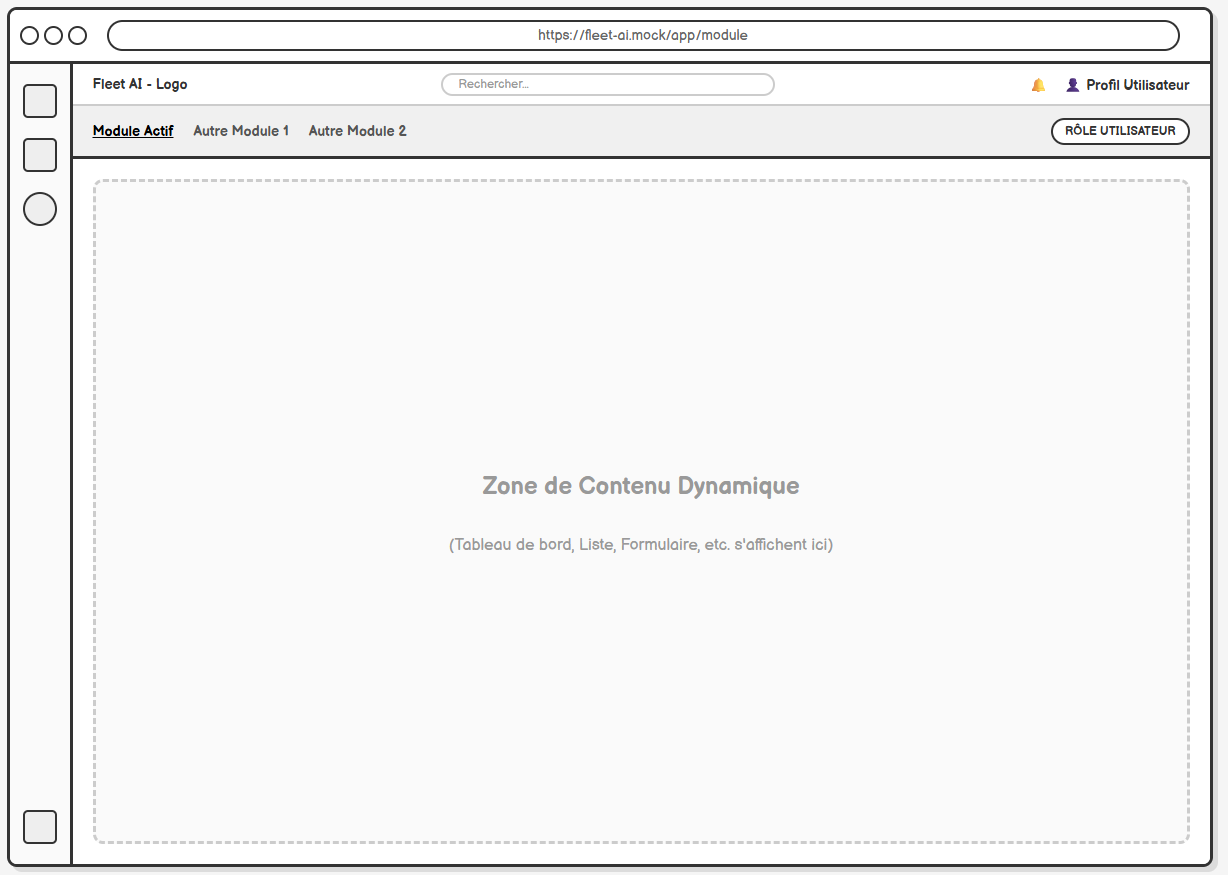
\includegraphics[width=0.9\linewidth, height=0.36\textheight, keepaspectratio]{img/maquette/maquette_layout_commun}
\caption{Maquette du layout commun de l'application}
\label{fig:maquette-layout-commun}
\end{figure}

\begin{figure}[H]
\centering
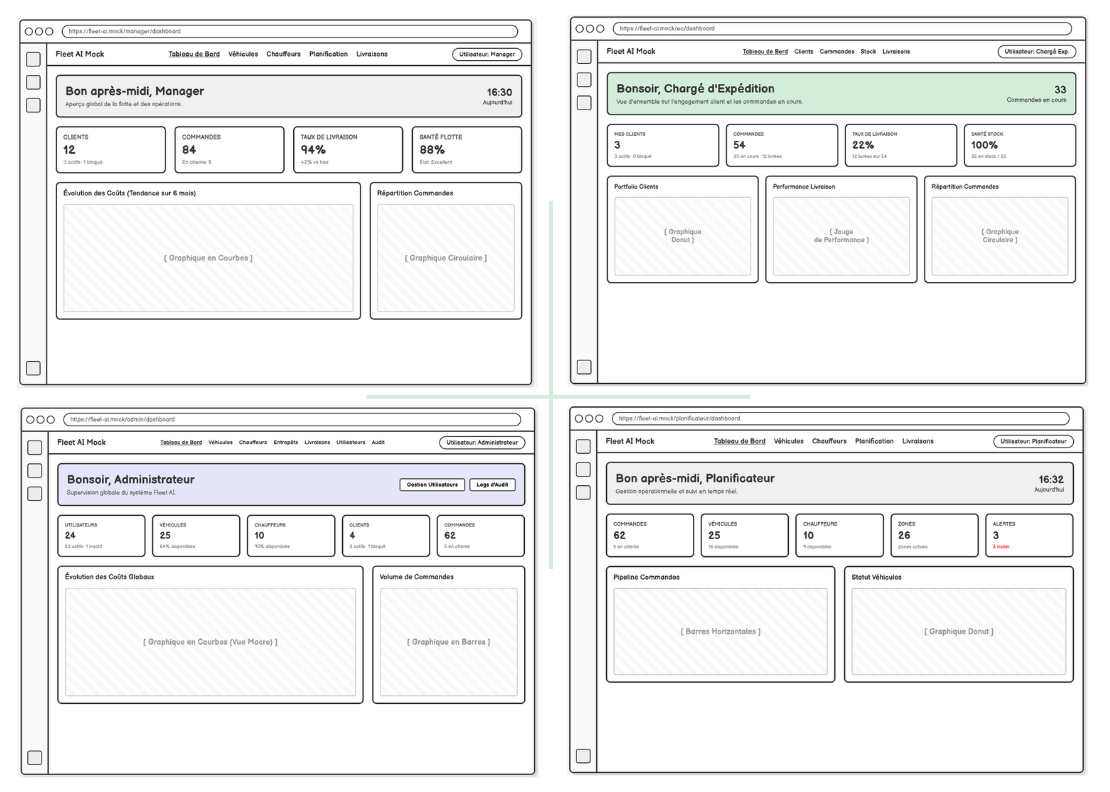
\includegraphics[width=0.9\linewidth, height=0.36\textheight, keepaspectratio]{img/maquette/maquette_dashboards}
\caption{Maquette de l'interface du tableau de bord}
\label{fig:maquette-dashboard}
\end{figure}

\begin{figure}[H]
\centering
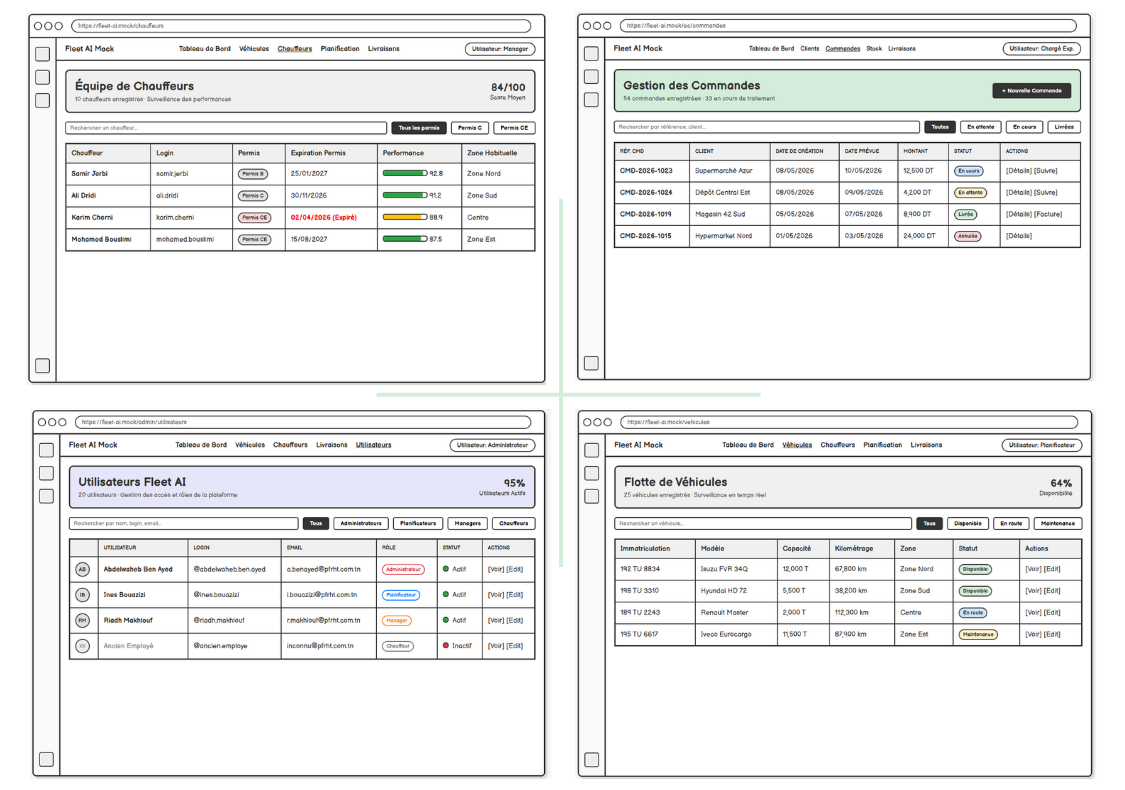
\includegraphics[width=0.9\linewidth, height=0.36\textheight, keepaspectratio]{img/maquette/maquette_desListes}
\caption{Maquette des interfaces de listes de données}
\label{fig:maquette-listes}
\end{figure}

\begin{figure}[H]
\centering
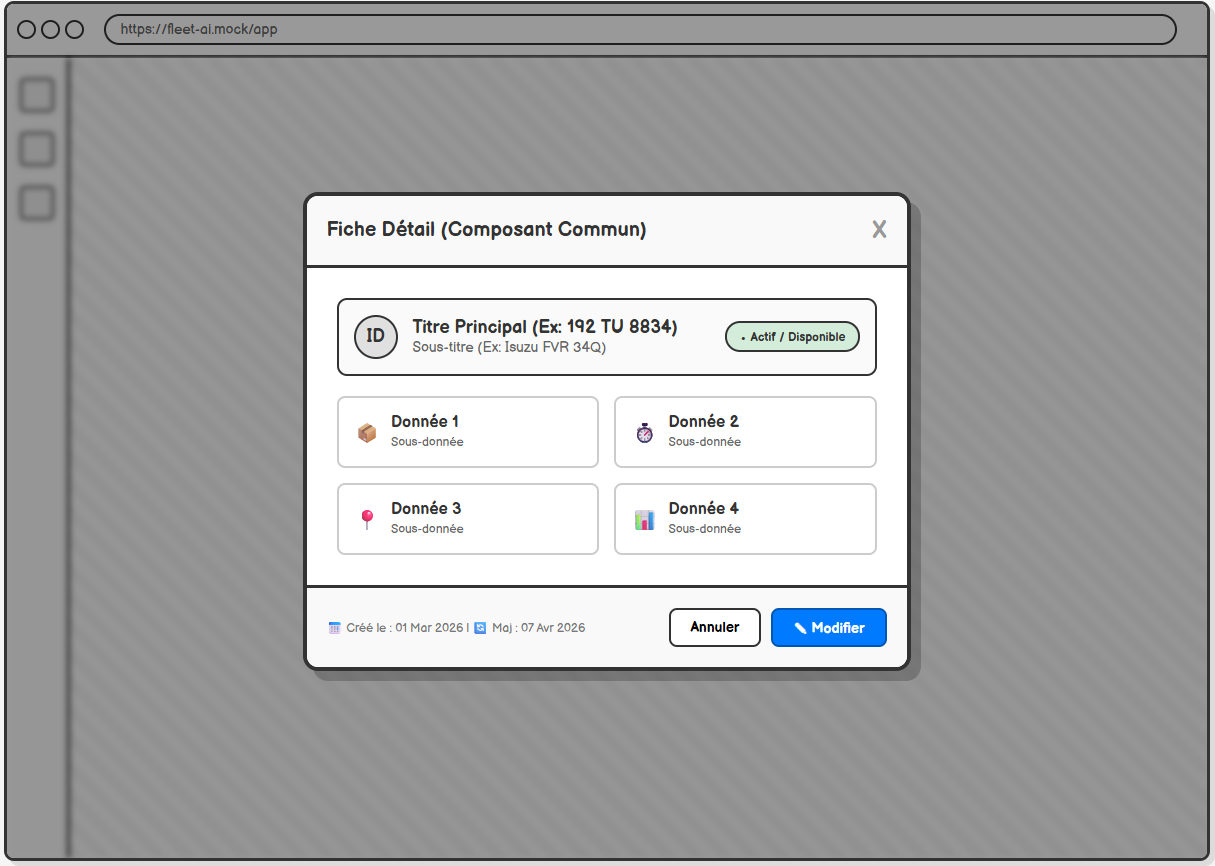
\includegraphics[width=0.9\linewidth, height=0.36\textheight, keepaspectratio]{img/maquette/maquette_modifier}
\caption{Maquette de l'interface de modification d'entité}
\label{fig:maquette-modifier}
\end{figure}

\begin{figure}[H]
\centering
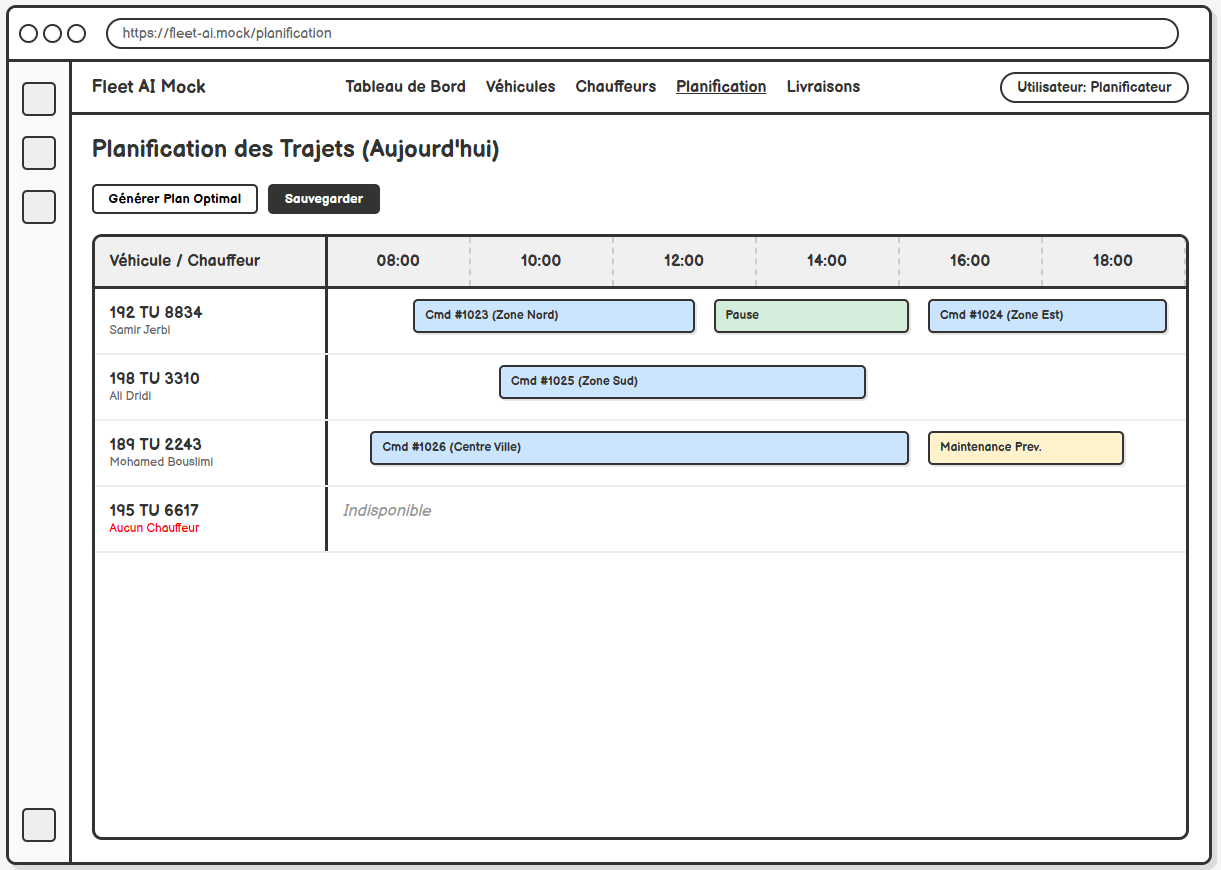
\includegraphics[width=0.9\linewidth, height=0.36\textheight, keepaspectratio]{img/maquette/maquette_disponibilite_desChauffeurs}
\caption{Maquette de l'interface de disponibilité des chauffeurs}
\label{fig:maquette-chauffeurs}
\end{figure}

\begin{figure}[H]
\centering
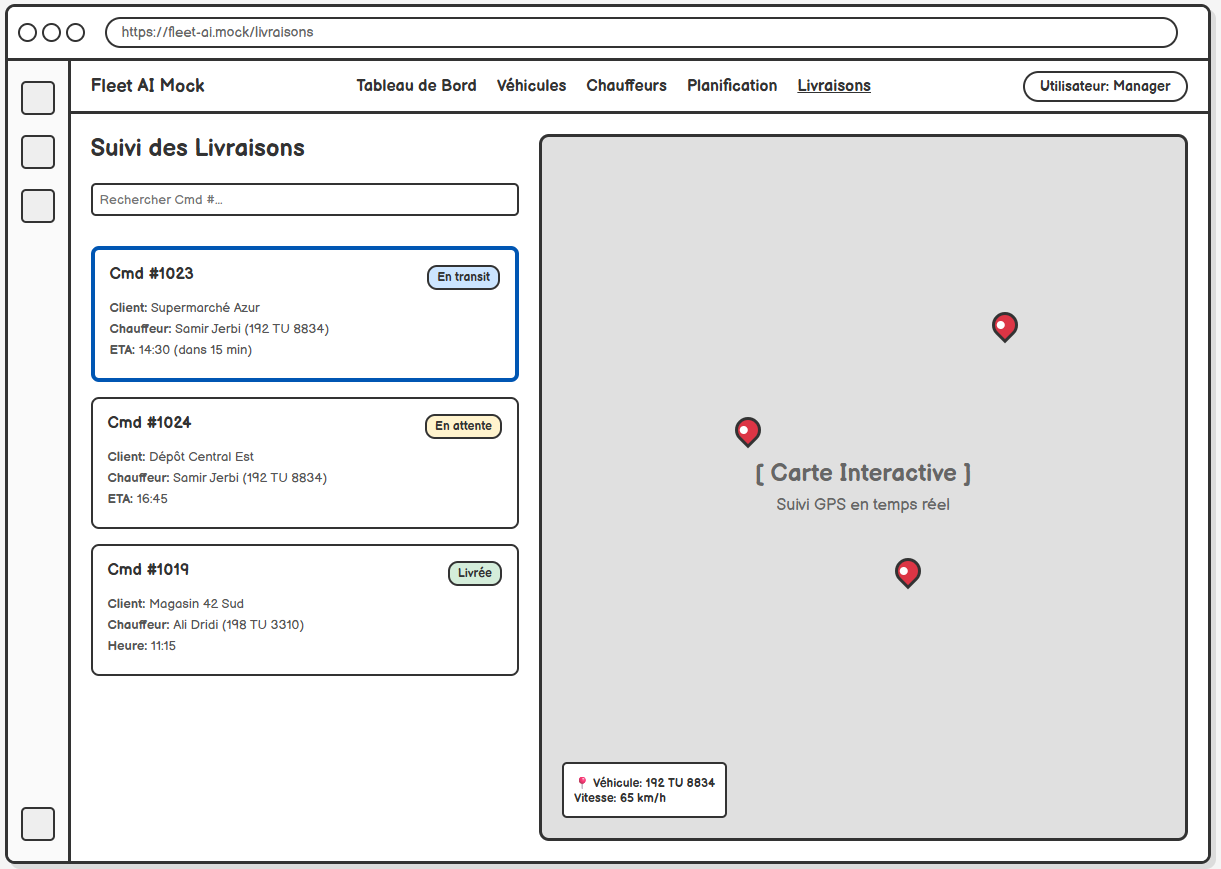
\includegraphics[width=0.9\linewidth, height=0.36\textheight, keepaspectratio]{img/maquette/maquette_suivi_livraison_endirect}
\caption{Maquette de la page de suivi des livraisons en direct}
\label{fig:maquette-planification}
\end{figure}

\subsection{Technologies à utiliser}

Le tableau ci-dessous liste les technologies retenues pour Fleet~AI.

\setlength{\arrayrulewidth}{1pt}
\begin{longtable}{|>{\raggedright\arraybackslash}p{4cm}|>{\raggedright\arraybackslash}p{3.5cm}|>{\raggedright\arraybackslash}p{7.5cm}|}
\hline
\rowcolor{headerbg}
\textbf{Technologie} & \textbf{Domaine} & \textbf{Rôle dans le projet} \\
\hline
\endfirsthead
\hline
\rowcolor{headerbg}
\textbf{Technologie} & \textbf{Domaine} & \textbf{Rôle dans le projet} \\
\hline
\endhead
\hline
\endfoot

Angular 19 + PrimeNG & Interface web & Application web Fleet~AI intégrée à la plateforme WFMS existante. \\
\hline
Flutter / Dart & Application mobile & Application mobile chauffeur et client (Android et iOS). \\
\hline
Spring Boot 3.4 & Backend & Services métier, API REST, sécurité et persistance des données. \\
\hline
Python / Flask & Passerelle & Passerelle WFMS existante gérant l'authentification centralisée. \\
\hline
Python / FastAPI & Service IA & Microservice dédié à l'optimisation des itinéraires et à la prédiction. \\
\hline
PostgreSQL & Base de données & Données structurées (utilisateurs, véhicules, commandes, paiements). \\
\hline
MongoDB & Base de données & Journaux d'audit applicatifs. \\
\hline
Redis & Cache & Mise en cache des données fréquemment consultées (KPIs, ressources). \\
\hline

\caption{Technologies retenues pour le projet Fleet~AI}
\end{longtable}
\setlength{\arrayrulewidth}{0.4pt}

\subsection{Contrainte technique : intégration WFMS et ERP}

Fleet~AI est une \textbf{application additionnelle} qui s'exécute dans un écosystème technique existant et en production. Cette contrainte impose deux règles architecturales non négociables.

\textbf{Intégration avec WFMS :}
\begin{itemize}[leftmargin=2.5em]
    \item[$\bullet$] Toutes les requêtes vers Fleet~AI transitent par la \textbf{passerelle Flask} de WFMS, qui gère l'authentification, le déchiffrement des tokens RSA et le routage.
    \item[$\bullet$] Le RBAC de Fleet~AI est aligné sur le système de rôles WFMS : AD, PL, MG, CH, REC, CL.
    \item[$\bullet$] L'interface Angular de Fleet~AI est intégrée dans la navigation latérale WFMS, avec le même thème PrimeNG et les mêmes mécanismes de session.
\end{itemize}

\textbf{Intégration avec l'ERP Poulina :}
\begin{itemize}[leftmargin=2.5em]
    \item[$\bullet$] Fleet~AI lit le stock réel depuis l'ERP via un adaptateur ETL en quasi temps réel.
    \item[$\bullet$] Quand une commande est acceptée dans Fleet~AI, elle est transmise à l'ERP pour préparation. L'ERP retourne le statut \textit{Prête} quand la commande est disponible pour l'affectation.
    \item[$\bullet$] Fleet~AI ne modifie pas le fonctionnement interne de l'ERP.
\end{itemize}

\subsection{Durée du projet}

Le projet a été réalisé sur une période de 4 mois (Février -- Mai 2025), organisée en cinq sprints de deux semaines.

\subsection{Livrables du projet}

À l'issue de ces travaux de conception et de développement, les livrables finaux fournis à GREPSYS et PGH sont structurés comme suit :
\begin{itemize}[leftmargin=2.5em]
    \item[$\bullet$] \textbf{Le code source complet :} L'ensemble du code backend (Spring Boot, FastAPI) et frontend (Angular).
    \item[$\bullet$] \textbf{L'application web :} Interface d'administration et de gestion déployée et intégrée au WFMS.
    \item[$\bullet$] \textbf{L'application mobile :} L'application Flutter (Android/iOS) destinée aux chauffeurs et aux clients.
    \item[$\bullet$] \textbf{Les modèles IA :} Les modèles de Machine Learning entraînés pour la prédiction et l'assistant conversationnel.
    \item[$\bullet$] \textbf{La documentation technique :} Les manuels d'architecture, de déploiement et d'utilisation de la plateforme.
    \item[$\bullet$] \textbf{La présentation du projet :} Support de présentation destiné à l'équipe logistique de PGH pour l'adoption du système.
\end{itemize}

\section*{Conclusion}
\addcontentsline{toc}{section}{Conclusion}
Ce chapitre a présenté GREPSYS Tunisia, Poulina Group Holding et le cahier des charges complet de Fleet~AI, incluant les fonctionnalités, les maquettes, les contraintes d'intégration WFMS/ERP et les livrables du projet. Le chapitre suivant analyse les solutions de gestion de flotte disponibles sur le marché et explique pourquoi aucune ne répond au besoin de PGH.
